
% ////////////////////////////////////////////////

\begin{titlepage}
    \begin{figure}[H]
    \centering
    \begin{subfigure}{0.18\textwidth} 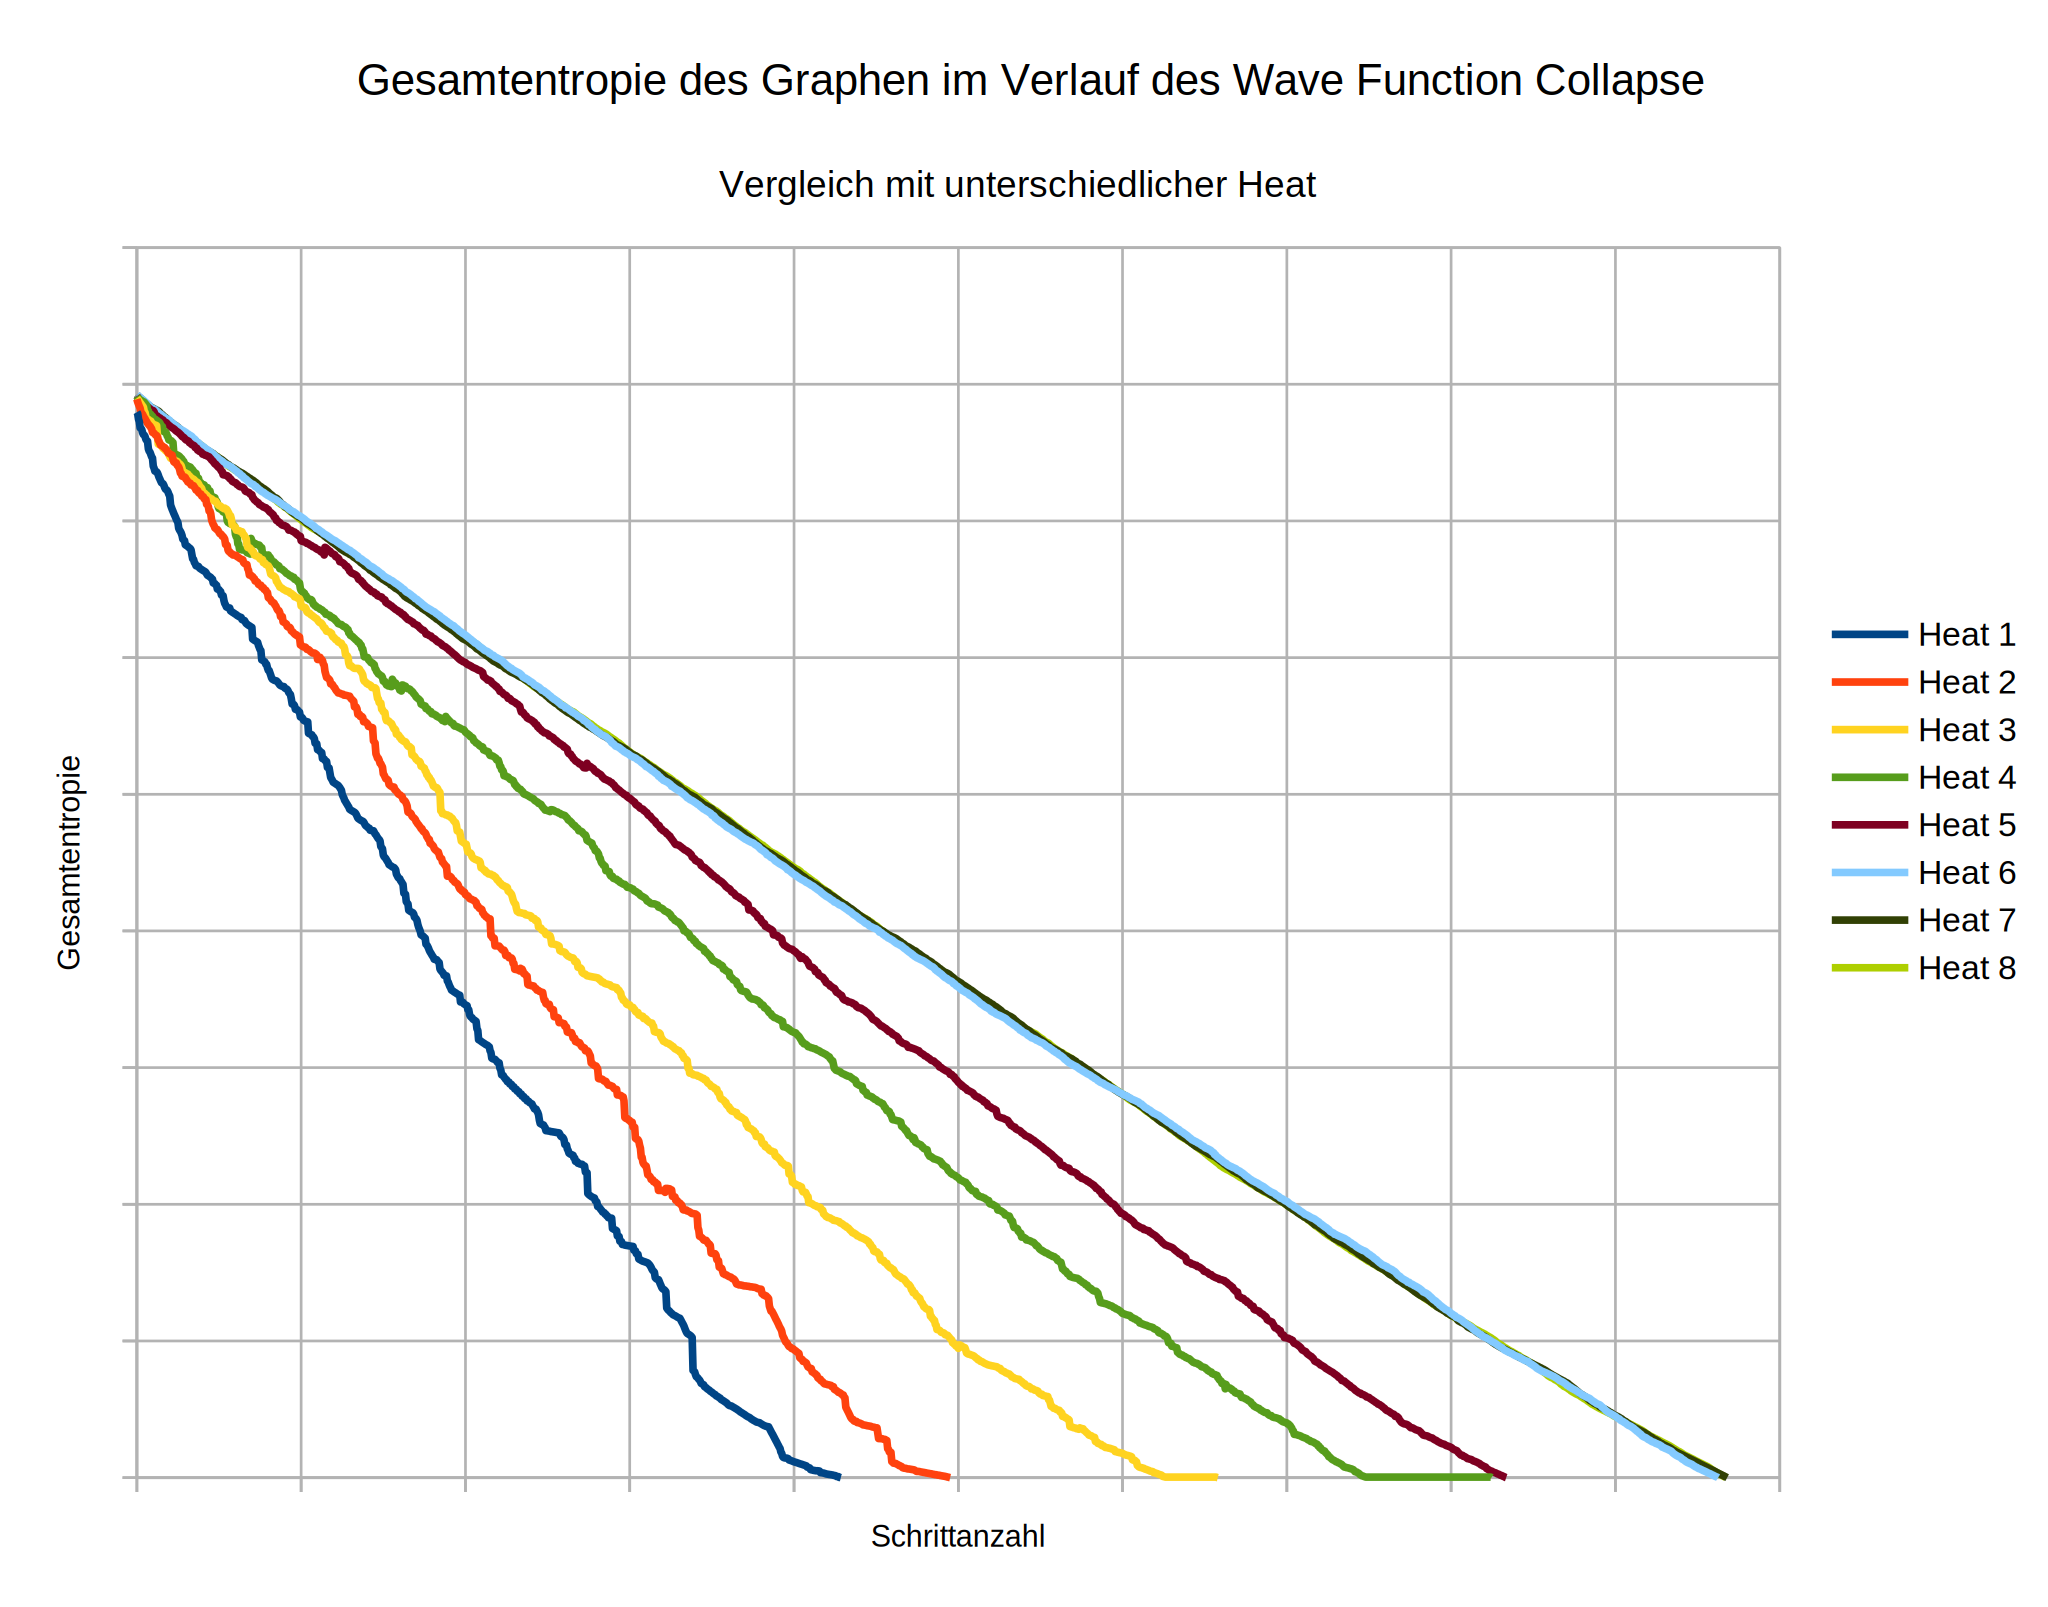
\includegraphics[width=\linewidth]{data/townscaper_grid/1.png} \caption{} \end{subfigure}
    \begin{subfigure}{0.18\textwidth} \includegraphics[width=\linewidth]{data/townscaper_grid/2.png} \caption{} \end{subfigure}
    \begin{subfigure}{0.18\textwidth} \includegraphics[width=\linewidth]{data/townscaper_grid/3.png} \caption{} \end{subfigure}
    \begin{subfigure}{0.18\textwidth} \includegraphics[width=\linewidth]{data/townscaper_grid/4.png} \caption{} \end{subfigure}
    \begin{subfigure}{0.18\textwidth} \includegraphics[width=\linewidth]{data/townscaper_grid/5.png} \caption{} \end{subfigure}
    
    \caption{
        Generierung eines Teils des Gitters für Townscaper \cite{stalberg_grid}. (a) Punkte werden generiert. (b) Triangulierung. (c) Kanten werden gelöscht, so dass Vierecke entstehen. (d) die Vierecke werden geviertelt. (e) Position der Knoten wird aufgelockert, so dass die Winkel zwischen Kanten gleichmäßiger sind.
    }
    \label{fig:townscaper_grid}
\end{figure}
    
    \begin{verbatim}
        
        
    \end{verbatim}
    
    \begin{center}
        \Large{Hochschule Anhalt}\\
        \Large{Fachbereich Informatik und Sprachen}\\
    \end{center}
    
    \begin{verbatim}
        
        
    \end{verbatim}
        
    \begin{center}
        \doublespacing
        \textbf{\LARGE{Bachelorarbeit}}\\
        \begin{verbatim}
            
        \end{verbatim}
        \textbf{\LARGE{Wave Function Collapse auf Graphen}}\\
        \singlespacing
        \begin{verbatim}
            
        \end{verbatim}
    \end{center}
    \begin{verbatim}
        
        
        
    \end{verbatim}
    \begin{flushleft}
        \begin{tabular}{llll}
            \textbf{Studiengang:} & & Angewandet Informatik: Digitale Medien und Spieleentwicklung & \\
            & & \\
            \textbf{Autor:} & & Name: Viktor Graf von Westarp & \\
            & & Matrikelnummer: 5058639 & \\
            & & E-Mail: viktor.grafvonwestarp@student.hs-anhalt.de & \\
            & & \\
            \textbf{Abgabedatum:} & & 5.\,Dezember\,2025 &\\
            & & \\
            \textbf{Betreuer:} & & Prof.\,Dr.\,Stefan Schlechtweg &\\
            \textbf{Zweitgutachterin:} & & Prof.\,Dr.\,Anika Groß &\\
        \end{tabular}
    \end{flushleft}
\end{titlepage}



% ////////////////////////////////////////////////

\tableofcontents

% ////////////////////////////////////////////////



\chapter*{Zusammenfassung}
\begin{quote}

Es wird eine Erweiterung des \textit{Wave Function Collapse} Algorithmus, die aus einem Beispiel ähnliche Ausgaben nicht nur wie zuvor auf regelmäßigen Gittern, sondern nun auch auf beliebigen Graphen, prozedural generieren kann, präsentiert. 
Die unterliegenden Struktur der Ausgabe wird von der Struktur des Beispiel entkoppelt und es können komplexere oder gar zuvor unmögliche, Ausgaben erstellt werden, ohne dass das Beispiel für diese angepasst werden muss. 
Ein neues Konzept namens \textit{Heat} definiert wie der Algorithmus die, aus dem Beispiel extrahierten, Regeln auf die Knoten des Graphen und deren Nachbarknoten anwendet. Dadurch können die Knoten beliebig angeordnet werden, anstatt auf ein Gitter beschränkt zu sein. Desweiteren wird Backtracking in der Generierung eingeführt, um die Laufzeit zu verbessern. Es wird auch gezeigt wie die, für die Ausgabe genutzten, Graphen automatisch erzeugt werden.
Der erweiterte Algorithmus kann mit dem selben Beispiel erfolgreich eine Vielzahl an Ausgaben auf unterschiedlichen Graphen generieren. Die Qualität der generierten Ausgabe hängt in gleichen Teilen von dem Beispiel, dem Graphen und der gewählten Heat ab. Diese Beziehung wird genauer untersucht.
Es wurde sich auf zweidimensionale Graphen beschränkt. Außerdem ist Heat als globaler, graphweiter Wert definiert. Dies macht die Methode besonders geeignet für Graphen mit relativ gleichmäßig verteilten Knoten. Bei stark unregelmäßige Graphstrukturen scheitert der Algorithmus häufiger oder kann nie eine zufriedenstellende Ausgabe generieren.

\end{quote}






\chapter{Einleitung}
    Diese Kapitel erklärt zuerst die Motivation hinter dieser Arbeit und geht auf das zulösende Problem und das genaue Ziel dieser Arbeit ein. Danach wird ein Überblick den Aufbau der Arbeit gegeben.
    
    \section{Motivation}
        Wave Function Collapse ist ein spannender Algorithmus, welcher, basiert auf einem einzigen Beispielmodell oder -bild, eine große Menge an ähnlichen Modellen und Bildern prozedural generieren kann. Bisher bestimmte die Form des Beispiels auch die Form des Ausgabe. Ein Beispielbild besteht aus Pixeln also werden auch Bilder aus Pixels generiert. Auch bei 3D Modellen beschränkt sich der Nutzer meist auf  z.B. würfelförmige Bauteile aus denen dann einen Modell zusammengestellt wird. Auch wenn der Innebereich solcher Bauteil beliebige Formen haben kann, werden die Bauteile dennoch würfelartig aneinander gebaut.
        
        Es muss aber nicht so sein, denn der Algorithmus selbst ist agnostisch gegenüber der Form der Ein- und Ausgabe. Es können nicht nur Bilder, sondern auch 3D Modelle generiert werden. Es sollte also möglich sein, dass der Algorithmus die Muster in einem Beispielbild auch auf eine anders geformte Struktur replizieren kann. Genauer sollten die Ausgabe nicht nur auf einem Gitter, sondern nun auch auf Graphen, geschehen können.
        
        Wäre dies möglich, so könnten Nutzer mit dem Algorithmus beliebige Strukturen als Basis nutzen und wären nicht mehr auf reine Gitter beschränkt. Dadurch könnten unregelmäßige oder organische Anordnungen, wie sind in der Natur, historischen Städten oder einem Mosaik vorkommen, als Basis für Ausgaben genutzt werden.
    
    
    
    \section{Problemstellung und Ziel}
        Ziel dieser Arbeit ist es, den Wave Function Collapse Algorithmus so erweitern, dass dieser eine Ausgabe auf Graphen generieren kann. Das heißt, dass die Struktur der Eingabe nicht mehr exakt zur Struktur der Ausgabe passen muss, sondern dass z.B. ein Beispielbild auf unterschiedlich strukturierte Graphen anwendbar sein soll, ohne dass das Beispielbild dafür verändert werden muss. 
        
        Das Kernproblem dabei ist, wie genau der Algorithmus die Informationen aus dem Beispielbild auf die Knoten eine Graphens einheitlich anwenden kann, wenn die Anordnung der Knoten und der Anzahl der Kanten pro Knoten im Graphen stark variieren können und keinerlei Ähnlichkeit zu dem Pixelgitter eines Bilds haben müssen. Gleichzeitig sollte der erweiterte Algorithmus immernoch die selbe Qualität für Ausgaben auf Gittern, als spezielle Art von Graphen, beibehalten. Insgesamt sollen die generierten Ausgaben eine gewisse Ähnlichkeit zum Beispiel haben, wobei diese vielleicht abgeschwächt werden muss. Dennoch sollte der Algorithmus eine hohe Ähnlichkeit erzielen.
    
    
    
    \section{Aufbau der Arbeit}
        Es folgen fünf Kapitel in dieser Arbeit. Zuerst werden grundlegende Begriffe erklärt und es wird ein Überblick über den Stand der Technik im Bereich Wave Function Collapse gegeben. Danach wird die Beschränkung des Algorithmus genauer beschrieben und darauf eingegangen wie der Algorithmus erweitert wird und welchen Änderungen es dafür bedarf. Danach wird erklärt wie diese Änderungen umgesetzt wurden. Es folgt ein Überblick über die erzielten Resultate und es wird genauer auf Aspekte der Erweiterung eingegangen. Schließlich folgt eine Zusammenfassung der Arbeit, in der auch auf die Vor- und die Nachteile genannt werden.



